\documentclass[aspectratio=169]{beamer}
\usetheme{Madrid}
\usecolortheme{default}

\usepackage{amsmath}
\usepackage{amssymb}
\usepackage{tikz}
\usepackage{pgfplots}
\pgfplotsset{compat=1.17}

\title{Derivative Tests, Convexity \& Inflection Points}
\author{Mathematics for ML}
\date{\today}

\begin{document}

\frame{\titlepage}

\begin{frame}{Outline}
\tableofcontents
\end{frame}

\section{First-Derivative Test}

\begin{frame}{First-Derivative Test: Concept}
\textbf{Purpose:} Identify local extrema (maxima and minima) using the first derivative.

\vspace{0.5cm}

\textbf{Critical Points:} Points where $f'(x) = 0$ or $f'(x)$ does not exist.

\vspace{0.5cm}

\textbf{First-Derivative Test:}
\begin{itemize}
    \item If $f'(x)$ changes from \textcolor{blue}{positive to negative} at $x = c$, then $f$ has a \textbf{local maximum} at $c$.
    \item If $f'(x)$ changes from \textcolor{red}{negative to positive} at $x = c$, then $f$ has a \textbf{local minimum} at $c$.
    \item If $f'(x)$ does not change sign at $x = c$, then $f$ has \textbf{no local extremum} at $c$.
\end{itemize}
\end{frame}

\begin{frame}{First-Derivative Test: Visual Interpretation}
\begin{center}
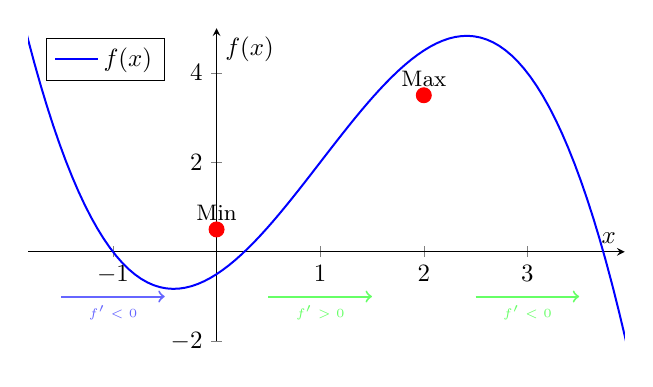
\begin{tikzpicture}[scale=0.9]
\begin{axis}[
    axis lines=middle,
    xlabel={$x$},
    ylabel={$f(x)$},
    domain=-2:4,
    samples=100,
    width=10cm,
    height=6cm,
    ymin=-2, ymax=5,
    legend pos=north west
]
\addplot[blue, thick] {-0.5*(x-1)^3 + 3*(x-1) + 2};
\addlegendentry{$f(x)$}

% Mark critical points
\addplot[red, only marks, mark=*, mark size=3pt] coordinates {(0, 0.5) (2, 3.5)};
\node[above] at (axis cs:0, 0.5) {\small Min};
\node[above] at (axis cs:2, 3.5) {\small Max};

% Add arrows showing derivative sign
\draw[->, thick, blue!60] (axis cs:-1.5, -1) -- (axis cs:-0.5, -1) node[midway, below] {\tiny $f' < 0$};
\draw[->, thick, green!60] (axis cs:0.5, -1) -- (axis cs:1.5, -1) node[midway, below] {\tiny $f' > 0$};
\draw[->, thick, green!60] (axis cs:2.5, -1) -- (axis cs:3.5, -1) node[midway, below] {\tiny $f' < 0$};
\end{axis}
\end{tikzpicture}
\end{center}
\textbf{Observation:} Derivative changes sign at extrema.
\end{frame}

\begin{frame}{Example 1: First-Derivative Test}
\textbf{Problem:} Find and classify the critical points of $f(x) = x^3 - 3x^2 - 9x + 5$.

\vspace{0.3cm}

\textbf{Solution:}
\begin{enumerate}
    \item Find $f'(x)$:
    $$f'(x) = 3x^2 - 6x - 9 = 3(x^2 - 2x - 3) = 3(x-3)(x+1)$$
    
    \item Critical points: $f'(x) = 0 \Rightarrow x = -1$ or $x = 3$
    
    \item Test intervals:
    \begin{itemize}
        \item $x < -1$: $f'(-2) = 15 > 0$ \quad (\textcolor{green}{increasing})
        \item $-1 < x < 3$: $f'(0) = -9 < 0$ \quad (\textcolor{red}{decreasing})
        \item $x > 3$: $f'(4) = 15 > 0$ \quad (\textcolor{green}{increasing})
    \end{itemize}
    
    \item \textbf{Conclusion:}
    \begin{itemize}
        \item $x = -1$: Local maximum (sign changes + to -)
        \item $x = 3$: Local minimum (sign changes - to +)
    \end{itemize}
\end{enumerate}
\end{frame}

\begin{frame}{Example 1: Visualization}
\begin{center}
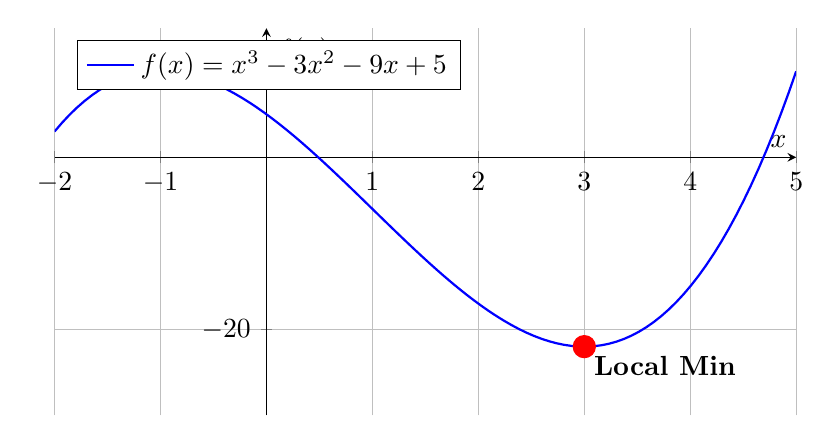
\begin{tikzpicture}
\begin{axis}[
    axis lines=middle,
    xlabel={$x$},
    ylabel={$f(x)$},
    domain=-2:5,
    samples=100,
    width=11cm,
    height=6.5cm,
    ymin=-30, ymax=15,
    grid=major,
    legend pos=north west
]
\addplot[blue, thick] {x^3 - 3*x^2 - 9*x + 5};
\addlegendentry{$f(x) = x^3 - 3x^2 - 9x + 5$}

% Mark critical points
\addplot[red, only marks, mark=*, mark size=4pt] coordinates {(-1, 10) (3, -22)};
\node[above right] at (axis cs:-1, 10) {\textbf{Local Max}};
\node[below right] at (axis cs:3, -22) {\textbf{Local Min}};
\end{axis}
\end{tikzpicture}
\end{center}
\end{frame}

\section{Second-Derivative Test}

\begin{frame}{Second-Derivative Test: Concept}
\textbf{Purpose:} Classify critical points using the second derivative (faster than first-derivative test).

\vspace{0.5cm}

\textbf{Second-Derivative Test:}

Let $c$ be a critical point where $f'(c) = 0$. Then:
\begin{itemize}
    \item If $f''(c) > 0$, then $f$ has a \textbf{local minimum} at $c$ \quad (concave up)
    \item If $f''(c) < 0$, then $f$ has a \textbf{local maximum} at $c$ \quad (concave down)
    \item If $f''(c) = 0$, the test is \textbf{inconclusive} (use first-derivative test)
\end{itemize}

\vspace{0.5cm}

\textbf{Intuition:} 
\begin{itemize}
    \item $f''(x) > 0$: function is \textcolor{blue}{curving upward} $\Rightarrow$ minimum
    \item $f''(x) < 0$: function is \textcolor{red}{curving downward} $\Rightarrow$ maximum
\end{itemize}
\end{frame}

\begin{frame}{Second-Derivative Test: Visual}
\begin{center}
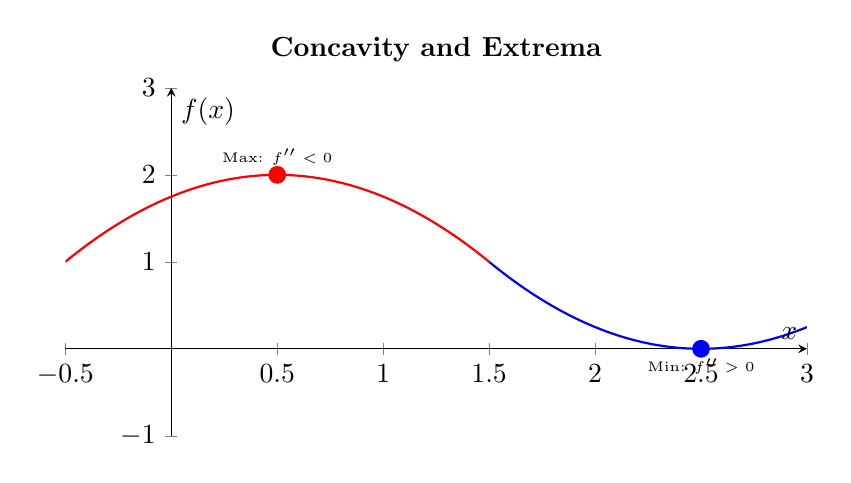
\begin{tikzpicture}
\begin{axis}[
    axis lines=middle,
    xlabel={$x$},
    ylabel={$f(x)$},
    domain=-1:3,
    samples=100,
    width=11cm,
    height=6cm,
    ymin=-1, ymax=3,
    title={\textbf{Concavity and Extrema}}
]
% Local maximum (concave down)
\addplot[red, thick, domain=-0.5:1.5] {2 - (x-0.5)^2};
\addplot[red, only marks, mark=*, mark size=3pt] coordinates {(0.5, 2)};
\node[above] at (axis cs:0.5, 2) {\tiny Max: $f''<0$};

% Local minimum (concave up)
\addplot[blue, thick, domain=1.5:3] {(x-2.5)^2};
\addplot[blue, only marks, mark=*, mark size=3pt] coordinates {(2.5, 0)};
\node[below] at (axis cs:2.5, 0) {\tiny Min: $f''>0$};
\end{axis}
\end{tikzpicture}
\end{center}
\end{frame}

\begin{frame}{Example 2: Second-Derivative Test}
\textbf{Problem:} Use the second-derivative test to classify critical points of $f(x) = x^4 - 4x^3 + 4x^2$.

\vspace{0.3cm}

\textbf{Solution:}
\begin{enumerate}
    \item Find $f'(x)$:
    $$f'(x) = 4x^3 - 12x^2 + 8x = 4x(x^2 - 3x + 2) = 4x(x-1)(x-2)$$
    Critical points: $x = 0, 1, 2$
    
    \item Find $f''(x)$:
    $$f''(x) = 12x^2 - 24x + 8$$
    
    \item Evaluate $f''$ at critical points:
    \begin{itemize}
        \item $f''(0) = 8 > 0$ \quad $\Rightarrow$ \textbf{Local minimum}
        \item $f''(1) = 12 - 24 + 8 = -4 < 0$ \quad $\Rightarrow$ \textbf{Local maximum}
        \item $f''(2) = 48 - 48 + 8 = 8 > 0$ \quad $\Rightarrow$ \textbf{Local minimum}
    \end{itemize}
\end{enumerate}
\end{frame}

\begin{frame}{Example 2: Visualization}
\begin{center}
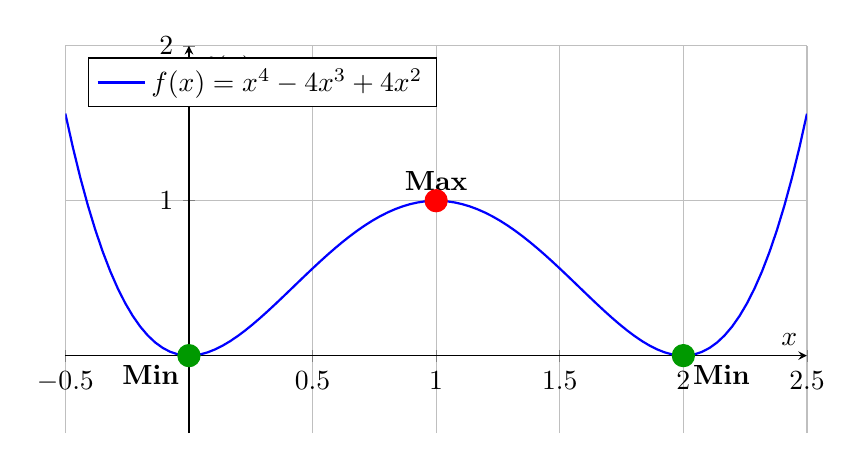
\begin{tikzpicture}
\begin{axis}[
    axis lines=middle,
    xlabel={$x$},
    ylabel={$f(x)$},
    domain=-0.5:2.5,
    samples=100,
    width=11cm,
    height=6.5cm,
    ymin=-0.5, ymax=2,
    grid=major,
    legend pos=north west
]
\addplot[blue, thick] {x^4 - 4*x^3 + 4*x^2};
\addlegendentry{$f(x) = x^4 - 4x^3 + 4x^2$}

% Mark critical points
\addplot[green!60!black, only marks, mark=*, mark size=4pt] coordinates {(0, 0) (2, 0)};
\addplot[red, only marks, mark=*, mark size=4pt] coordinates {(1, 1)};
\node[below left] at (axis cs:0, 0) {\textbf{Min}};
\node[above] at (axis cs:1, 1) {\textbf{Max}};
\node[below right] at (axis cs:2, 0) {\textbf{Min}};
\end{axis}
\end{tikzpicture}
\end{center}
\end{frame}

\section{Convexity and Concavity}

\begin{frame}{Convex and Concave Functions}
\textbf{Definitions:}
\begin{itemize}
    \item $f$ is \textbf{concave up (convex)} on interval $I$ if $f''(x) > 0$ for all $x \in I$
    \item $f$ is \textbf{concave down (concave)} on interval $I$ if $f''(x) < 0$ for all $x \in I$
\end{itemize}

\vspace{0.5cm}

\textbf{Geometric Interpretation:}
\begin{columns}
\column{0.5\textwidth}
\textbf{Convex (Concave Up):}
\begin{itemize}
    \item Curves upward
    \item Tangent lines below curve
    \item $f''(x) > 0$
\end{itemize}

\column{0.5\textwidth}
\textbf{Concave (Concave Down):}
\begin{itemize}
    \item Curves downward
    \item Tangent lines above curve
    \item $f''(x) < 0$
\end{itemize}
\end{columns}

\vspace{0.5cm}

\textbf{Alternative Definition (Secant Line):}
$f$ is convex if for all $x_1, x_2$ and $\lambda \in [0,1]$:
$$f(\lambda x_1 + (1-\lambda)x_2) \leq \lambda f(x_1) + (1-\lambda)f(x_2)$$
\end{frame}

\begin{frame}{Convexity vs Concavity: Visual Comparison}
\begin{center}
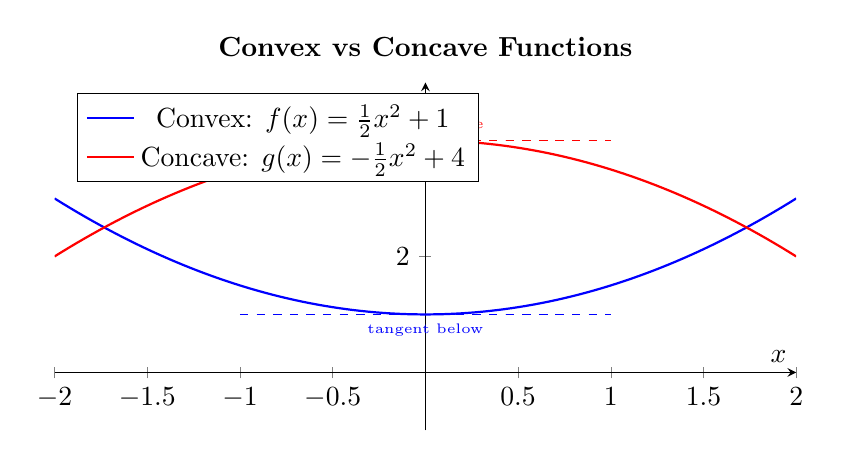
\begin{tikzpicture}
\begin{axis}[
    axis lines=middle,
    xlabel={$x$},
    ylabel={},
    domain=-2:2,
    samples=100,
    width=11cm,
    height=6cm,
    ymin=-1, ymax=5,
    legend pos=north west,
    title={\textbf{Convex vs Concave Functions}}
]
% Convex function
\addplot[blue, thick] {0.5*x^2 + 1};
\addlegendentry{Convex: $f(x) = \frac{1}{2}x^2 + 1$}

% Concave function
\addplot[red, thick] {-0.5*x^2 + 4};
\addlegendentry{Concave: $g(x) = -\frac{1}{2}x^2 + 4$}

% Tangent line for convex
\addplot[blue, dashed, domain=-1:1] {1 + 0*x};
\node[blue, below] at (axis cs:0, 1) {\tiny tangent below};

% Tangent line for concave
\addplot[red, dashed, domain=-1:1] {4 + 0*x};
\node[red, above] at (axis cs:0, 4) {\tiny tangent above};
\end{axis}
\end{tikzpicture}
\end{center}
\end{frame}

\begin{frame}{Example 3: Determine Convexity}
\textbf{Problem:} Determine where $f(x) = x^3 - 6x^2 + 9x + 1$ is convex and concave.

\vspace{0.3cm}

\textbf{Solution:}
\begin{enumerate}
    \item Find $f''(x)$:
    $$f'(x) = 3x^2 - 12x + 9$$
    $$f''(x) = 6x - 12 = 6(x - 2)$$
    
    \item Find where $f''(x) = 0$:
    $$6(x - 2) = 0 \Rightarrow x = 2$$
    
    \item Test intervals:
    \begin{itemize}
        \item For $x < 2$: $f''(1) = -6 < 0$ \quad $\Rightarrow$ \textbf{Concave down}
        \item For $x > 2$: $f''(3) = 6 > 0$ \quad $\Rightarrow$ \textbf{Concave up (Convex)}
    \end{itemize}
\end{enumerate}

\vspace{0.3cm}

\textbf{Conclusion:}
\begin{itemize}
    \item Concave on $(-\infty, 2)$
    \item Convex on $(2, \infty)$
    \item Point $x = 2$ is an \textbf{inflection point}
\end{itemize}
\end{frame}

\section{Inflection Points}

\begin{frame}{Inflection Points: Definition}
\textbf{Definition:} A point $x = c$ is an \textbf{inflection point} if:
\begin{enumerate}
    \item The concavity of $f$ changes at $x = c$
    \item Equivalently: $f''(x)$ changes sign at $x = c$
\end{enumerate}

\vspace{0.5cm}

\textbf{Finding Inflection Points:}
\begin{enumerate}
    \item Find $f''(x)$
    \item Solve $f''(x) = 0$ (or find where $f''$ doesn't exist)
    \item \textbf{Verify} that $f''$ changes sign at these points
\end{enumerate}

\vspace{0.5cm}

\textbf{Warning:} $f''(c) = 0$ does NOT guarantee an inflection point!
\begin{itemize}
    \item Example: $f(x) = x^4$ has $f''(0) = 0$, but $x = 0$ is \textbf{not} an inflection point
    \item $f''(x) = 12x^2 \geq 0$ for all $x$ (no sign change)
\end{itemize}
\end{frame}

\begin{frame}{Inflection Points: Visual}
\begin{center}
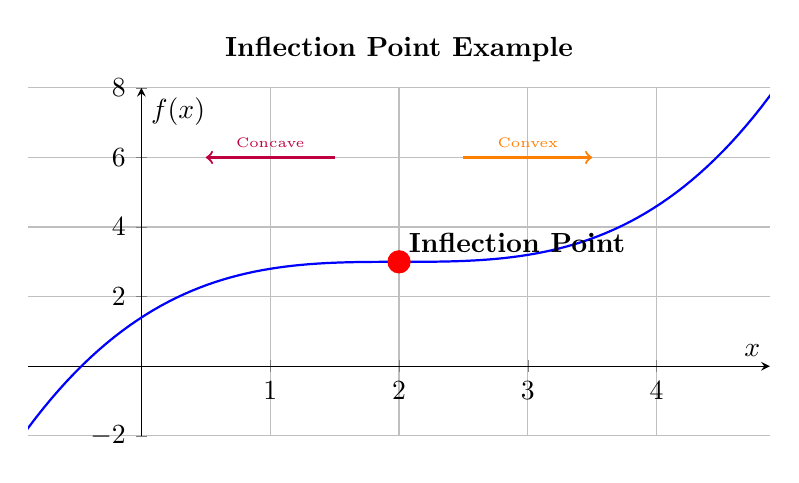
\begin{tikzpicture}
\begin{axis}[
    axis lines=middle,
    xlabel={$x$},
    ylabel={$f(x)$},
    domain=-1:5,
    samples=100,
    width=11cm,
    height=6cm,
    ymin=-2, ymax=8,
    grid=major,
    title={\textbf{Inflection Point Example}}
]
\addplot[blue, thick] {0.2*(x-2)^3 + 3};
\addplot[red, only marks, mark=*, mark size=4pt] coordinates {(2, 3)};
\node[above right] at (axis cs:2, 3) {\textbf{Inflection Point}};

% Show concavity regions
\draw[<-, thick, purple] (axis cs:0.5, 6) -- (axis cs:1.5, 6) node[midway, above] {\tiny Concave};
\draw[->, thick, orange] (axis cs:2.5, 6) -- (axis cs:3.5, 6) node[midway, above] {\tiny Convex};
\end{axis}
\end{tikzpicture}
\end{center}

At the inflection point, the curve changes from concave down to concave up (or vice versa).
\end{frame}

\begin{frame}{Example 4: Finding Inflection Points}
\textbf{Problem:} Find all inflection points of $f(x) = x^4 - 6x^3 + 12x^2 - 8x + 3$.

\vspace{0.3cm}

\textbf{Solution:}
\begin{enumerate}
    \item Find $f''(x)$:
    $$f'(x) = 4x^3 - 18x^2 + 24x - 8$$
    $$f''(x) = 12x^2 - 36x + 24 = 12(x^2 - 3x + 2) = 12(x-1)(x-2)$$
    
    \item Solve $f''(x) = 0$:
    $$12(x-1)(x-2) = 0 \Rightarrow x = 1 \text{ or } x = 2$$
    
    \item Check sign changes:
    \begin{itemize}
        \item $x < 1$: $f''(0) = 24 > 0$ \quad (convex)
        \item $1 < x < 2$: $f''(1.5) = -3 < 0$ \quad (concave)
        \item $x > 2$: $f''(3) = 24 > 0$ \quad (convex)
    \end{itemize}
\end{enumerate}

\textbf{Conclusion:} Inflection points at $x = 1$ and $x = 2$ (both have sign changes).
\end{frame}

\begin{frame}{Example 4: Visualization}
\begin{center}
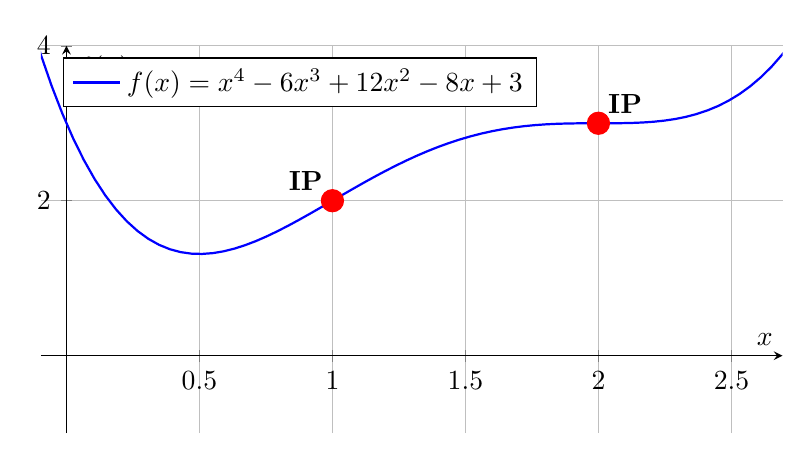
\begin{tikzpicture}
\begin{axis}[
    axis lines=middle,
    xlabel={$x$},
    ylabel={$f(x)$},
    domain=-0.5:3.5,
    samples=100,
    width=11cm,
    height=6.5cm,
    ymin=-1, ymax=4,
    grid=major,
    legend pos=north west
]
\addplot[blue, thick] {x^4 - 6*x^3 + 12*x^2 - 8*x + 3};
\addlegendentry{$f(x) = x^4 - 6x^3 + 12x^2 - 8x + 3$}

% Mark inflection points
\addplot[red, only marks, mark=*, mark size=4pt] coordinates {(1, 2) (2, 3)};
\node[above left] at (axis cs:1, 2) {\textbf{IP}};
\node[above right] at (axis cs:2, 3) {\textbf{IP}};

% Show concavity
\node[blue] at (axis cs:0.3, 3.5) {\tiny $f''>0$};
\node[red] at (axis cs:1.5, 3.5) {\tiny $f''<0$};
\node[blue] at (axis cs:3, 3.5) {\tiny $f''>0$};
\end{axis}
\end{tikzpicture}
\end{center}
\end{frame}

\section{Combined Example}

\begin{frame}{Comprehensive Example}
\textbf{Problem:} Analyze $f(x) = x^3 - 3x + 1$ completely:
\begin{itemize}
    \item Find critical points and classify them
    \item Determine concavity
    \item Find inflection points
\end{itemize}

\vspace{0.3cm}

\textbf{Solution:}
\begin{enumerate}
    \item \textbf{First derivative:} $f'(x) = 3x^2 - 3 = 3(x^2 - 1) = 3(x-1)(x+1)$
    \begin{itemize}
        \item Critical points: $x = -1, 1$
    \end{itemize}
    
    \item \textbf{Second derivative:} $f''(x) = 6x$
    
    \item \textbf{Classify critical points:}
    \begin{itemize}
        \item $f''(-1) = -6 < 0$ $\Rightarrow$ local maximum at $x = -1$, $f(-1) = 3$
        \item $f''(1) = 6 > 0$ $\Rightarrow$ local minimum at $x = 1$, $f(1) = -1$
    \end{itemize}
\end{enumerate}
\end{frame}

\begin{frame}{Comprehensive Example (continued)}
\begin{enumerate}
    \setcounter{enumi}{3}
    \item \textbf{Concavity:}
    \begin{itemize}
        \item $f''(x) = 6x$
        \item $x < 0$: $f''(x) < 0$ (concave down)
        \item $x > 0$: $f''(x) > 0$ (concave up / convex)
    \end{itemize}
    
    \item \textbf{Inflection point:}
    \begin{itemize}
        \item $f''(x) = 0 \Rightarrow x = 0$
        \item Sign changes from negative to positive
        \item Inflection point at $(0, f(0)) = (0, 1)$
    \end{itemize}
\end{enumerate}

\vspace{0.5cm}

\textbf{Summary:}
\begin{itemize}
    \item Local max at $(-1, 3)$
    \item Local min at $(1, -1)$
    \item Inflection point at $(0, 1)$
    \item Concave on $(-\infty, 0)$, convex on $(0, \infty)$
\end{itemize}
\end{frame}

\begin{frame}{Comprehensive Example: Complete Graph}
\begin{center}
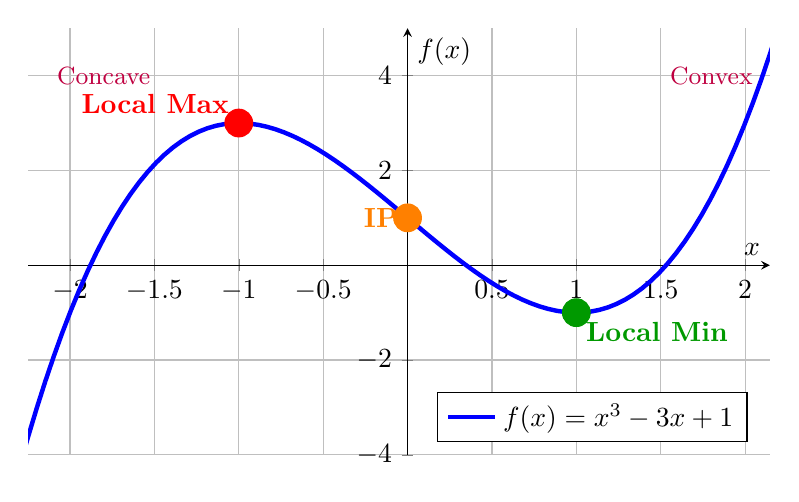
\begin{tikzpicture}
\begin{axis}[
    axis lines=middle,
    xlabel={$x$},
    ylabel={$f(x)$},
    domain=-2.5:2.5,
    samples=100,
    width=11cm,
    height=7cm,
    ymin=-4, ymax=5,
    grid=major,
    legend pos=south east
]
\addplot[blue, ultra thick] {x^3 - 3*x + 1};
\addlegendentry{$f(x) = x^3 - 3x + 1$}

% Mark critical points
\addplot[red, only marks, mark=*, mark size=5pt] coordinates {(-1, 3)};
\node[above left, red] at (axis cs:-1, 3) {\textbf{Local Max}};

\addplot[green!60!black, only marks, mark=*, mark size=5pt] coordinates {(1, -1)};
\node[below right, green!60!black] at (axis cs:1, -1) {\textbf{Local Min}};

% Mark inflection point
\addplot[orange, only marks, mark=*, mark size=5pt] coordinates {(0, 1)};
\node[left, orange] at (axis cs:0, 1) {\textbf{IP}};

% Show concavity regions
\node[purple] at (axis cs:-1.8, 4) {\small Concave};
\node[purple] at (axis cs:1.8, 4) {\small Convex};
\end{axis}
\end{tikzpicture}
\end{center}
\end{frame}

\section{Summary}

\begin{frame}{Summary Table}
\begin{table}
\centering
\small
\begin{tabular}{|l|l|l|}
\hline
\textbf{Concept} & \textbf{Condition} & \textbf{Interpretation} \\
\hline
\hline
\multicolumn{3}{|c|}{\textbf{First-Derivative Test}} \\
\hline
Critical point & $f'(c) = 0$ & Potential extremum \\
Local maximum & $f'$ changes + to - & Top of hill \\
Local minimum & $f'$ changes - to + & Bottom of valley \\
\hline
\hline
\multicolumn{3}{|c|}{\textbf{Second-Derivative Test}} \\
\hline
Local maximum & $f'(c) = 0, f''(c) < 0$ & Concave down at $c$ \\
Local minimum & $f'(c) = 0, f''(c) > 0$ & Concave up at $c$ \\
Inconclusive & $f'(c) = 0, f''(c) = 0$ & Use 1st derivative test \\
\hline
\hline
\multicolumn{3}{|c|}{\textbf{Concavity}} \\
\hline
Convex (Concave up) & $f''(x) > 0$ & Curves upward \\
Concave (Concave down) & $f''(x) < 0$ & Curves downward \\
\hline
\hline
\multicolumn{3}{|c|}{\textbf{Inflection Points}} \\
\hline
Inflection point & $f''$ changes sign & Concavity changes \\
\hline
\end{tabular}
\end{table}
\end{frame}

\begin{frame}{Key Relationships}
\begin{center}
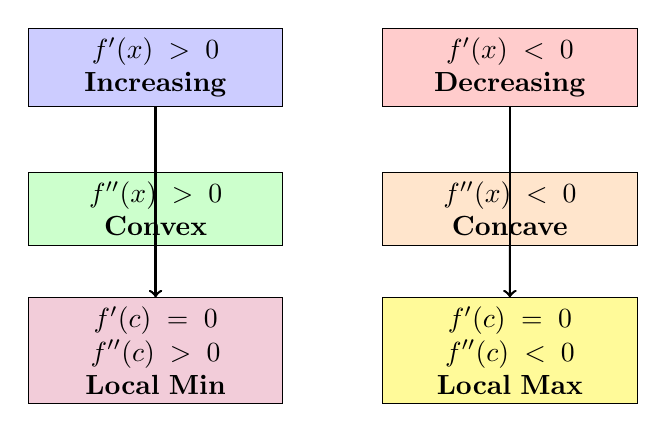
\begin{tikzpicture}[scale=0.9]
% First row
\node[draw, rectangle, fill=blue!20, text width=3cm, align=center] (f1) at (0, 4) {$f'(x) > 0$ \\ \textbf{Increasing}};
\node[draw, rectangle, fill=red!20, text width=3cm, align=center] (f2) at (5, 4) {$f'(x) < 0$ \\ \textbf{Decreasing}};

% Second row
\node[draw, rectangle, fill=green!20, text width=3cm, align=center] (f3) at (0, 2) {$f''(x) > 0$ \\ \textbf{Convex}};
\node[draw, rectangle, fill=orange!20, text width=3cm, align=center] (f4) at (5, 2) {$f''(x) < 0$ \\ \textbf{Concave}};

% Third row
\node[draw, rectangle, fill=purple!20, text width=3cm, align=center] (f5) at (0, 0) {$f'(c) = 0$ \\ $f''(c) > 0$ \\ \textbf{Local Min}};
\node[draw, rectangle, fill=yellow!40, text width=3cm, align=center] (f6) at (5, 0) {$f'(c) = 0$ \\ $f''(c) < 0$ \\ \textbf{Local Max}};

% Arrows
\draw[->, thick] (f1) -- (f5);
\draw[->, thick] (f3) -- (f5);
\draw[->, thick] (f2) -- (f6);
\draw[->, thick] (f4) -- (f6);
\end{tikzpicture}
\end{center}
\end{frame}

\begin{frame}{Practice Problems}
\textbf{Try these on your own:}

\vspace{0.3cm}

\begin{enumerate}
    \item Find and classify all critical points of $f(x) = x^4 - 4x^3 + 10$
    
    \item Determine the intervals where $g(x) = \frac{x^3}{3} - \frac{x^2}{2} - 2x + 1$ is convex and concave
    
    \item Find all inflection points of $h(x) = x^5 - 5x^4 + 5x^3$
    
    \item For $f(x) = xe^{-x}$:
    \begin{itemize}
        \item Find critical points
        \item Determine concavity
        \item Sketch the graph
    \end{itemize}
    
    \item Prove that $f(x) = \ln(x)$ is concave on $(0, \infty)$
\end{enumerate}
\end{frame}

\begin{frame}{Applications}
\textbf{Real-World Applications:}

\vspace{0.3cm}

\begin{itemize}
    \item \textbf{Economics:}
    \begin{itemize}
        \item Profit maximization (find where $\text{Profit}'(x) = 0$)
        \item Diminishing marginal returns (concavity of production functions)
        \item Cost minimization
    \end{itemize}
    
    \item \textbf{Machine Learning:}
    \begin{itemize}
        \item Loss function optimization
        \item Convex optimization ensures global minimum
        \item Second-order methods (Newton's method)
    \end{itemize}
    
    \item \textbf{Physics:}
    \begin{itemize}
        \item Maximum height of projectile
        \item Minimum energy states
    \end{itemize}
    
    \item \textbf{Data Analysis:}
    \begin{itemize}
        \item Finding peaks and valleys in time series
        \item Change point detection (inflection points)
    \end{itemize}
\end{itemize}
\end{frame}

\begin{frame}{}
\begin{center}
\Huge Thank You!

\vspace{1cm}

\Large Questions?

\vspace{1cm}

\normalsize
\textit{Remember: Derivatives tell us about rate of change,} \\
\textit{second derivatives tell us about the rate of change of the rate of change!}
\end{center}
\end{frame}

\end{document}
